\begin{frame}\frametitle{Background}
Main idea: train a network on a "fake task" then use the weights as embedding. \bigskip
\begin{itemize}
\item The fake task:
\item Given a word $w$ guess the context words. 
\item We want to maximize the following probability:
\end{itemize}
\begin{equation}
\prod_{t=1}^T \prod_{-m<j<m}  p(w_{t+j}|w_t)
\end{equation}
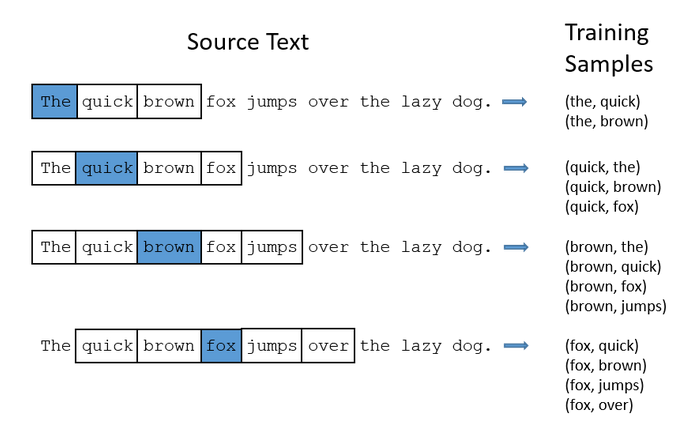
\includegraphics[scale=0.37]{images/context_pairs.pdf}
\end{frame}